\documentclass{article}

% Packages
\usepackage[english]{babel}
\usepackage[utf8]{inputenc}
\usepackage [autostyle]{csquotes}
\usepackage{graphicx}
\usepackage{tabularx}

\usepackage[style=authoryear]{biblatex} % Change "authoryear" to another style if preferred
\addbibresource{references.bib} % Link your .bib file

\newcommand{\chapsubhead}[1]{{\Large #1 \vspace{2ex}}}
\newcommand{\chaptype}[1]{{\Large \itshape (#1) \vspace{2ex}}}

\usepackage{graphicx}
\usepackage{pdfpages}
\usepackage{hyperref}
\usepackage{lipsum} % For generating dummy text, you can remove this package in your actual report

% Title, author, date
\title{Option Profit Calculator}
\author{Michael Martinez}
\date{December 17, 2024} % Or specify a specific date

\begin{document}

\maketitle

\section{Background}
\indent In the age of digital stock brokerages and low-to-no commission trading, individuals have been empowered to make a wide range of investments across equities, derivatives, and cryptocurrencies safely and efficiently. Tools to help traders keep track of their own portfolio and monitor future investments are widespread, but can be locked behind paywalls (e.g. Snowball Analytics) or only offer a very specific service. The goal of this project is to outline a centralized application with a user-friendly interface as a trading and portfolio analytics tool specifically for traders that use Charles Schwab as their brokerage. The project is implemented entirely in Python so as to open up the project to customization by users in the future. 

\indent In this project, I created two basic functionalities: 
\begin{enumerate}
    \item Interface to create an investment strategy based on different financial instruments.
    \item Given an investment strategy, the ability to simulate the possible profit/payoff that could occur in the future.
\end{enumerate}

The final product is an open-source GitHub repository that a user can easily clone into their own local machine, connect to their Charles Schwab brokerage account, and start the application on their machine to view their portfolio and chart investments. 

\indent A demo mode with dummy data is also available for users that do not have access to Charles Schwab. 

\indent This report will frequently use the term \enquote{option}, which is the name for a financial instrument that gives a buyer the option to buy or sell a stock or commodity. One stock or commodity can have hundreds of options contracts, even on the same day. These can be represented in an \enquote{options chain}, a tabular representation of all the options for one stock. Options have exploded in popularity recently because of their propensity for very high returns (or losses). They are also popular as a field of study in finance because of the mathematics that can be used to model their valuation. 

\indent Options can either be "calls" or "puts". Call options give the buyer the right to buy, or enter a long position on the underlying asset at an agreed price known as the "strike price". Put options give the buyer the right to sell, or short the underlying asset at the strike price. Options are not indefinite investments, having set expiration dates where the holder must exercise the option or accept a loss, depending on the final stock price of the underlying asset. Importantly, option contracts usually control $100$ shares of the asset, meaning that profit, loss, and cost must be multiplied by a factor of $100$.

\indent As an example, imagine a trader named John who speculates on Monday that Microsoft's stock will rise based on the company's earnings report on Wednesday. The current Microsoft stock price is $S=450$. He judges that it will increase to be greater than or equal to $S=455$ by the end of the week. He buys a call option with strike price of $K=455$ expiring by 4:00 pm on Friday. If John is correct, and $S_t\geq455$, then the option becomes "In the Money", and John has the opportunity to buy the underlying at $K=455$, regardless if $S_t > K$. This means that John receives a "discount" of $S_t-K \geq 0$, yielding the value of the option. We subtract the initial cost of the contract and multiply by $100$ to yield the final profit, $((S_t-K)-C_0)\times100$, where $C_0$ is the initial cost. If he is wrong, and $S_t < K$, then the option becomes "Out of the Money". If the option is "Out of the Money" by the market close on Friday, the contract becomes worthless, and his profit becomes $(0-C_0)\times 100$. We can make the call profit at expiration formula more concise: 
$$ C = [\max\{S_t-K,0\}-C_0]\times100$$
The logic is similar for put options: 
$$ P = [\max\{K-S_t,0\}-P_0]\times100$$
In other words, the put option is profitable if $S_t \leq K$ and $K-S_t-P_0 > 0$. A put option would make sense if John believed that Microsoft would have a poor earnings report. 

\indent We can visualize this function with payoff diagrams, with an example of a long call in Figure \ref{fig:Figure 1}. The x-axis represents the stock price, and the y-axis represents the profit of the option. The "bend" in the plot occurs when $S=K$, or the stock price reaches the strike price of the call. The constant line before $K$ represents the initial premium paid for the call. After the "bend", the call value increases 1:1 with the stock price. 

\indent Traders can also opt to be on the other side of the trade, selling, or "shorting" the option. An example of a short call can be found in Figure \ref{fig:Figure 2}. Notice here that the trade is initially positive, representing the premium gained by selling the option. After the "bend", the value decreases 1:1 with the stock price. As the stock price increases, the seller's loss can be unlimited. For this reason, short calls or short puts are generally not used alone, as they can be extremely risky. They are typically used alongside other options as part of advanced strategies. Note that while a long call is "bullish", meaning the trader profits if the stock rises above $K$, the short call is "bearish" where the trader profits if the stock falls $K$. On the flip side, long puts are "bearish", while short puts are "bullish". 

\begin{figure}[htbp]
    \centering
    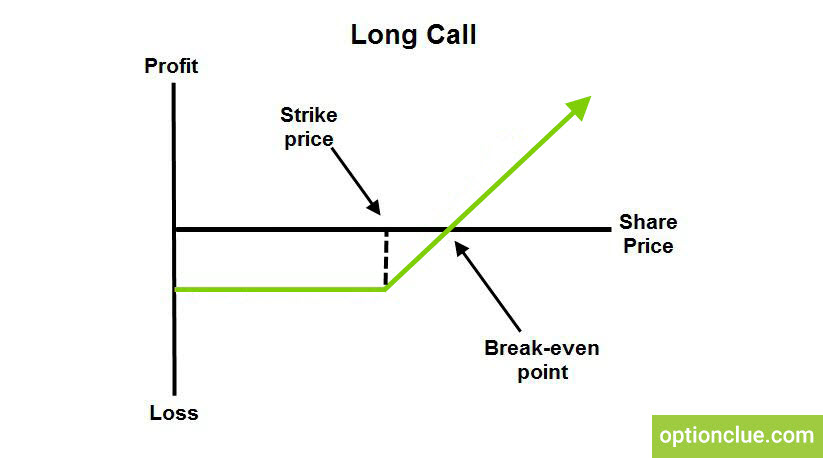
\includegraphics[width=1\textwidth]{assets/Long-Call.jpg}
    \caption{\label{fig:Figure 1}Long call payoff diagram (\cite{optionclue1}).}
\end{figure}

\begin{figure}[htbp]
    \centering
    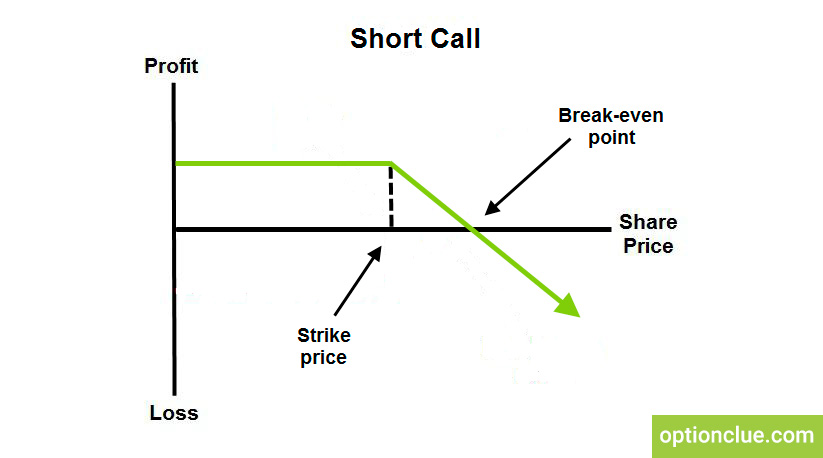
\includegraphics[width=1\textwidth]{assets/Short-Call.jpg}
    \caption{\label{fig:Figure 2}Short call payoff diagram (\cite{optionclue2}).}
\end{figure}

Traders often combine multiple options together to create more complicated strategies. An example can be found in Figure \ref{fig:Figure 3}, where a long call and a long put with the same strike price $K$ are combined to profit off of large positive or negative movement in the underlying asset. The goal of the Option Profit Calculator is to create a platform where these strategies can be created easily and their costs and profits can be visualized.  

\begin{figure}[htbp]
    \centering
    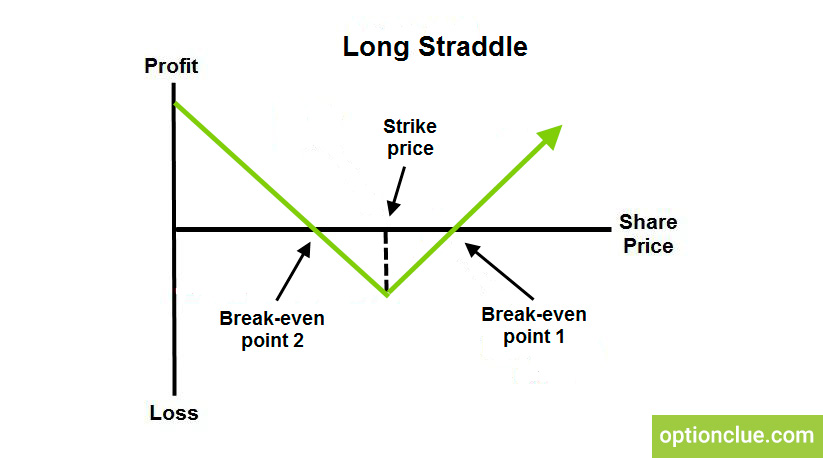
\includegraphics[width=1\textwidth]{assets/Straddle.jpg}
    \caption{\label{fig:Figure 3}Straddle payoff diagram (\cite{optionclue3}).}
\end{figure}

Another goal of the option profit calculator is to be able to model the future value of complex option strategies. Many mathematical models have been developed to model the valuation of European and American options in financial markets. The most well known is the Black-Sholes model, which models European options. According to the original formulation, for a call ($C$) and put ($P$), the premiums can be given by:  

$$
C = S_0 \Phi(d_1) - K e^{-rT} \Phi(d_2)
$$

$$
P = K e^{-rT} \Phi(-d_2) - S_0 \Phi(-d_1)
$$

where

$$
d_1 = \frac{\ln\left(\frac{S_0}{K}\right) + \left(r + \frac{\sigma^2}{2}\right)T}{\sigma \sqrt{T}}
$$

and

$$
d_2 = d_1 - \sigma \sqrt{T}
$$
where
\begin{itemize}
    \item $C$ = Price of the call option
    \item $P$ = Price of the put option
    \item $S_0$ = Current price of the underlying asset
    \item $K$ = Strike price of the option
    \item $r$ = Risk-free interest rate (in practice, U.S. treasury rate)
    \item $T$ = Time to expiration (in years)
    \item $\sigma$ = Volatility of the underlying asset (the expected movement)
    \item $\Phi$ = Cumulative distribution function of the standard normal distribution

\end{itemize}

The Black-Sholes formula is unfortunately only suited for pricing European options. This is because European options have the unique trait that the option is only able to be exercised at expiration. However, American options allow the holder to exercise at any time before expiration. In other words, if the holder wants to buy/sell the asset before the expiration date, and their option is \enquote{In-the-Money}, then they can do so. For American pricing models, this means that any time where it is more valuable to exercise the option by buying or selling the asset (as opposed to selling the option at its current value) must be accounted for. 

\indent In practice, this is usually done through numerical methods such as the Binomial/Trinomial Option Pricing Model, which essentially simulates every possible timestep between the current date and the expiration date and finds moments where it is optimal to exercise the option. However, the Option Profit Calculator uses a closed-form approximation called the Bjerksund-Stensland 2002 model to price American options (\cite{bjerksundstens}). 

% \indent To model future payoff, the Option Profit Calculator has a \enquote{Future Payoff} tab, which can be opened

% It can be useful to 

\section{Data Overview}

\indent All data is sourced using Schwab Developer (\cite{schwab_developer}), the official API for accessing market data through Charles Schwab's brokerage. To create a Schwab Developer account, you may follow these steps: 

\begin{itemize}
    \item Create a Schwab Developer account \href{https://developer.schwab.com/register}{here}. Note this account will be different than your Schwab brokerage/trading account, if you have one. 
    \item Once your account is created, navigate to the dashboard and click \enquote{Create App}
    \item Fill out the form to create an application. First, for "Select an API Product", add both \enquote{Accounts and Trading Production} and \enquote{Market Data Production} 
    \item Next, name the application (e.g. Derivatives Investment Tool)
    \item Add a short description (e.g. \enquote{Creating a tool to query market data to monitor my portfolio and chart investment strategies})
    \item Enter the callback URL: https://127.0.0.1 (this is the local host for your machine, and is used to get the necessary authentication tokens to access data)

\end{itemize}

\indent Once you have submitted the registration, Schwab Developer will approve your app for production. This usually takes 5-10 business days. Initially, the \enquote{Status} bar in the Dashboard will read \enquote{Approved - Pending}. Once it is approved, it will read \enquote{Ready For Use}. 

\indent Once the app is approved, you need to link your Schwab brokerage account with the Schwab Developer account. You can do this by following these steps: 
\begin{itemize}
    \item Clone the GitHub repository at this \href{https://github.com/mikemartinez13/option-profit-calculator}{link}.
    \item Use either \enquote{conda env create --name options-proj --file=options\_proj.yml} or \enquote{pip install -r requirements.txt} to install the necessary packages. 
    \item Navigate to your Schwab Developer dashboard. Click \enquote{View Details} on your created app, find the \enquote{App Key} and \enquote{Secret Key}, and copy them. These will enable you to authenticate. 
    \item Create a file named \enquote{.env} and format it like so: 
    \\ APP\_KEY = \enquote{Your App Key}
    \\ SECRET\_KEY = \enquote{Your Secret Key}
    \item Run ``main.py''. This will take you to an authentication site, where you will use your Charles Schwab brokerage credentials (not Schwab Developer) to login. 
    \item After you've agreed to the terms and conditions, click the trading accounts you would like to link with Schwab Developer. 
    \item Once you've given access to the trading accounts, you will be taken to an error screen. Copy the URL at the top of the error screen and paste it in the command line, where it reads "After authorizing, paste the address bar url here:"

\end{itemize}

\indent The raw format of the data provided by the Schwab Developer API is in JSON format. The API interface has multiple calls that allows the user to get quotes for stock, option data, personal account data, and more that can be accessed through the \enquote{requests} library in Python. An example of the output of a request is given in Figure~\ref{fig:Figure 4}.

\begin{figure}
    \begin{center}
    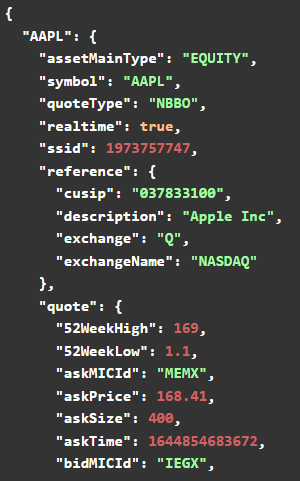
\includegraphics[scale=1]{example_quote.png}
    \caption{\label{fig:Figure 4}Raw output when requesting a quote for Apple stock.}
    \end{center}
\end{figure}



For more detailed information on data format, refer to the \href{https://developer.schwab.com/products/trader-api--individual/details/specifications/Market%20Data%20Production}{official Schwab Developer documentation} (Note you will need a Schwab Developer account to access this). 

\indent For the investment strategy builder, the code reorganizes the raw data into an options chain, which is displayed for the user to select the securities they would like to trade. An example of the options data is given in Figure~\ref{fig:Figure 5} (note the data has been split into two tables here for clarity): 


\begin{figure}[h]
    \centering

    \resizebox{\textwidth}{!}{%
    \begin{tabular}{lllllllll}
      & Contract Name         & Description             & Strike & Bid    & Ask    & Last   & Mark   & Delta \\
    0 & AAPL  241115C00005000 & AAPL 11/15/2024 5.00 C  & 5.0    & 221.35 & 222.85 & 0.0    & 222.1  & 1.0   \\
    1 & AAPL  241115C00010000 & AAPL 11/15/2024 10.00 C & 10.0   & 216.85 & 218.3  & 217.5  & 217.58 & 1.0   \\
    2 & AAPL  241115C00015000 & AAPL 11/15/2024 15.00 C & 15.0   & 211.85 & 213.3  & 212.95 & 212.58 & 1.0   \\
    3 & AAPL  241115C00020000 & AAPL 11/15/2024 20.00 C & 20.0   & 206.85 & 207.35 & 202.6  & 207.1  & 1.0   \\
    4 & AAPL  241115C00025000 & AAPL 11/15/2024 25.00 C & 25.0   & 201.8  & 202.85 & 202.1  & 202.33 & 1.0   \\
    5 & AAPL  241115C00030000 & AAPL 11/15/2024 30.00 C & 30.0   & 196.85 & 198.35 & 202.45 & 197.6  & 1.0   \\
    6 & AAPL  241115C00035000 & AAPL 11/15/2024 35.00 C & 35.0   & 191.85 & 192.85 & 0.0    & 192.35 & 1.0   \\
    7 & AAPL  241115C00040000 & AAPL 11/15/2024 40.00 C & 40.0   & 186.85 & 188.35 & 188.05 & 187.6  & 1.0   \\
    8 & AAPL  241115C00045000 & AAPL 11/15/2024 45.00 C & 45.0   & 180.0  & 183.25 & 0.0    & 181.63 & 1.0   \\
    9 & AAPL  241115C00050000 & AAPL 11/15/2024 50.00 C & 50.0   & 176.85 & 177.8  & 177.63 & 177.33 & 1.0  
    \end{tabular}%
    }
    \resizebox{\textwidth}{!}{%
    \begin{tabular}{lllllllll}
      & Gamma & Theta  & Vega & Rho   & ITM  & Intrinsic Value & Extrinsic Value & Days to Expiration \\
    0 & 0.0   & -0.019 & 0.0  & 0.001 & True & 221.96          & -221.96         & 6                  \\
    1 & 0.0   & -0.02  & 0.0  & 0.002 & True & 216.96          & 0.54            & 6                  \\
    2 & 0.0   & -0.021 & 0.0  & 0.003 & True & 211.96          & 0.99            & 6                  \\
    3 & 0.0   & -0.022 & 0.0  & 0.004 & True & 206.96          & -4.36           & 6                  \\
    4 & 0.0   & -0.022 & 0.0  & 0.005 & True & 201.96          & 0.14            & 6                  \\
    5 & 0.0   & -0.023 & 0.0  & 0.006 & True & 196.96          & 5.49            & 6                  \\
    6 & 0.0   & -0.023 & 0.0  & 0.007 & True & 191.96          & -191.96         & 6                  \\
    7 & 0.0   & -0.024 & 0.0  & 0.008 & True & 186.96          & 1.09            & 6                  \\
    8 & 0.0   & -0.025 & 0.0  & 0.009 & True & 181.96          & -181.96         & 6                  \\
    9 & 0.0   & -0.025 & 0.0  & 0.01  & True & 176.96          & 0.67            & 6                 
    \end{tabular}%
    }
    \caption{Example of an options chain.}
    \label{fig:Figure 5}
\end{figure}

Users here will be able to view key details about the different options they can choose for one expiration date. The \enquote{Contract Name} and \enquote{Description} columns give information about the official name of the option as well as key details about the underlying stock, expiration date, strike price, and type of option (\enquote{call} or \enquote{put}). The \enquote{Bid}, \enquote{Ask}, \enquote{Last}, and \enquote{Mark} columns give information about the current market price of the option. The \enquote{Delta}, \enquote{Gamma}. \enquote{Theta}, \enquote{Vega}, and \enquote{Rho} columns give technical details of how the value of the option changes with respect to different market factors, such as stock volatility or interest rates. The \enquote{ITM}, column stands for \enquote{In-the-Money}, which is a Boolean value that indicates whether the option can be exercised in the current moment or not. The \enquote{Intrinsic Value} column denotes the current value of an option when taking the difference between its strike price and the current stock price of the underlying asset. The \enquote{Extrinsic Value} represents the value of the option not made up by the Intrinsic Value, or in other words, the value of the option attributed to market factors such as volatility or specific excitement over a certain stock. Finally, the \enquote{Days to Expiration} column represents the time until the contract expires, when the value of the option becomes worthless.  

\section{Methods}

\indent The Option Profit Calculator is modularized into separate PyQt5 components that open different windows, each serving a separate function. A high-level overview of each component's relation to each other can be found in Figure \ref{fig:Figure 6}. The main.py file serves to only call the MainWindow, and it is not a window in itself. The MainWindow serves as a welcome page for the user, giving a short description of the project and its functionality, and giving the user the option to select to \enquote{Build Strategy} and \enquote{View Portfolio}. The Portfolio Viewer is still in development, so the button has been disabled. Clicking the Strategy Builder button connects to a function in window.py that instantiates the OptionChainWindow class, which inherits from the QWidget base class. This starts up the Strategy Builder window, which is described by the OptionChainWindow. 

\begin{figure}
    \begin{center}
    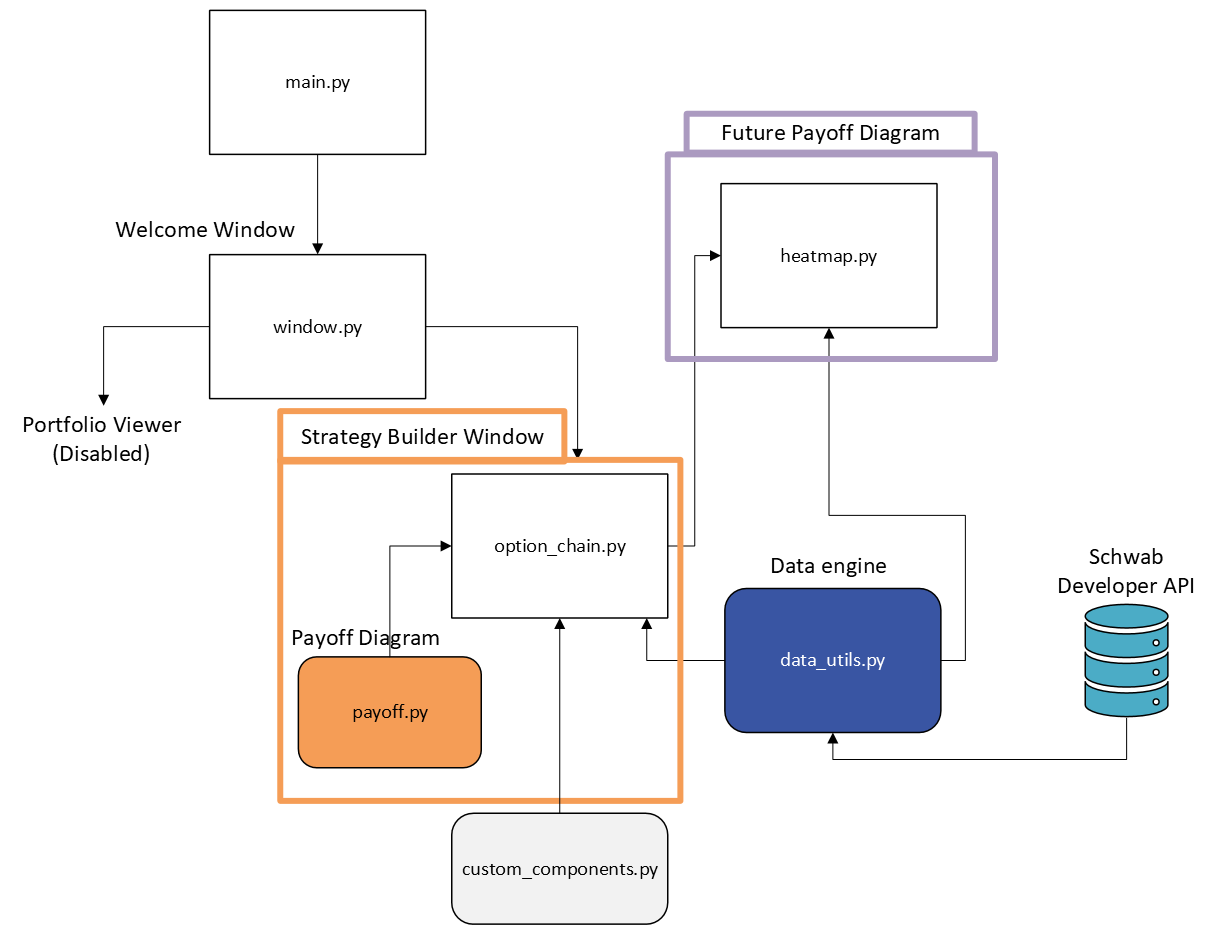
\includegraphics[width=\textwidth,height=\textheight,keepaspectratio]{assets/opc-diagram.png}
    \caption{\label{fig:Figure 6}Flowchart relating each component in the Option Profit Calculator.}
    \end{center}
\end{figure}

\indent The OptionChainWindow is the the main window that allows users to query options and add them to their strategy. To query data from the Schwab Developer API, it creates the SchwabData class sourced from data\_utils.py as its \enquote{engine} that powers data querying. If the user runs the app in demo mode, then the DummyData class is called instead. The SchwabData has methods to read the user's API key, call an option chain based on the ticker a user inputs, filter it into Pandas DataFrame format, and return it as a dictionary, with one key for the calls DataFrame and one key for the puts DataFrame. The SchwabData class makes use of the schwabdev package (\cite{schwabdev}), which simplifies querying from the API. 

\indent When the user inputs a ticker, OptionChainWindow sends the ticker to SchwabData, which returns the dictionary of data. Along with the dictionary of calls and puts, SchwabData returns information about the market, including the current interest rate, the current stock price of the ticker, and the current dividend price of the ticker, which the OptionChainWindow saves as attributes and uses to populate the window and to populate the DataFrame in the middle of the window as well as all of its tabs. The DataFrame is a custom PyQt5 object based on (reference) that is designed to render DataFrames and allow interactivity for the user. Calls are rendered by default, but if the user clicks the \enquote{Toggle Calls/Puts} button, the DataFrame will repopulate with puts by accessing the data attribute. When the user clicks on a observation in the DataFrame, the OptionChainWindow stores the clicked option as an attribute, which lets it be aware of the right option to add to the user's strategy when they click \enquote{Add Long to Plot} or \enquote{Add Short to Plot}. 

\indent To plot options, the OptionChainWindow instantiates the OptionPayoffPlot class from payoff.py as its \enquote{display}. Once a user clicks the Add Long or Add Short buttons, the OptionChainWindow handles the clicks by calling the \enquote{add\_option} in the display object, which is designed to take in the individual option data in dictionary format. In addition, once these buttons are first clicked, If there is no previous option on the plot, the display instantiates the data as an attribute; if there is, the display adds the new option data onto the old one to create a combined position. This data is then rendered into a PlotWidget object from the Pyqtgraph library, which is a graphing library specifically designed to work with PyQt5. As the user clicks Add Long or Add Short and adds options to their strategy, the option data displayed on the left side of the OptionChainWindow is updated accordingly. If the user clicks \enquote{Reset Plot}, all option data is cleared. If the user changes the ticker, then a warning is given notifying the user that all option data as well as stock information will be cleared if they proceed. 

\indent Once a user has added options to their strategy, the \enquote{Show Future Payoff} button will be enabled. Once this button is clicked, a Heatmap object sourced from heatmap.py takes in all the current options that the user has added as well as information about the current stock price, interest rate, and dividend yield. It then calculates the value of the option over a range of stock prices and a range of dates leading up to the expiration date (for strategies with options having multiple different expiration dates, it takes the largest expiration date). This calculation is performed using the Bjkersund-Stensland 2002 model developed in the optlib package (\cite{optlib}). This data is displayed in a heatmap, showing detailed information about where the option strategy yields profit in the future. It's important to note that the calculation assumes all other parameters $(K, r, \sigma, d)$ remain constant, which is not generally guaranteed, especially for volatility $(\sigma)$. The user is also able to change the range of the stock prices. 



\section{Output}

\indent The final PyQt5 application is able to query data from the Schwab Developer API relatively fast and renders plots accurately. An example of the Strategy Builder window without data can be found in Figure \ref{fig:Figure 7}. Customizing the theme, font, and color scheme was fairly simple, but customizing the specific layout to be eye-appealing to the user and make use of white space effectively was particularly challenging in PyQt5. 

\begin{figure}[htbp]
    \centering
    \makebox[\textwidth]{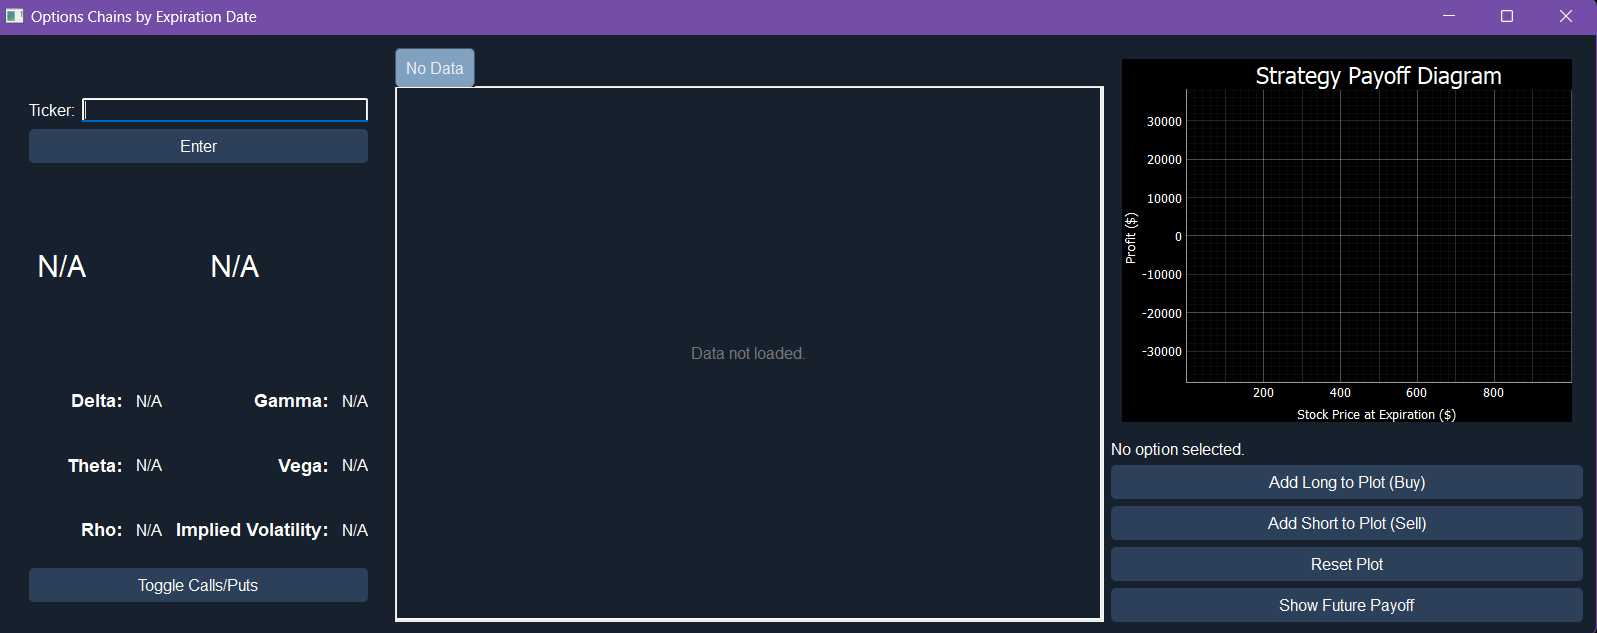
\includegraphics[width=1.4\textwidth]{assets/strategy-builder-empty.png}}
    \caption{\label{fig:Figure 7}Initial rendering of the Strategy Builder window without data.}
\end{figure}

In the top-left corner, the ticker input box, which is a PyQt5 QLabel, allows the user to input the ticker symbol for a desired stock. Pressing "Enter" will populate the middle DataFrame with the options chain for the stock. An example loading data for Microsoft (MSFT) can be found in Figure \ref{fig:Figure 8}

\begin{figure}[htbp]
    \centering
    \makebox[\textwidth]{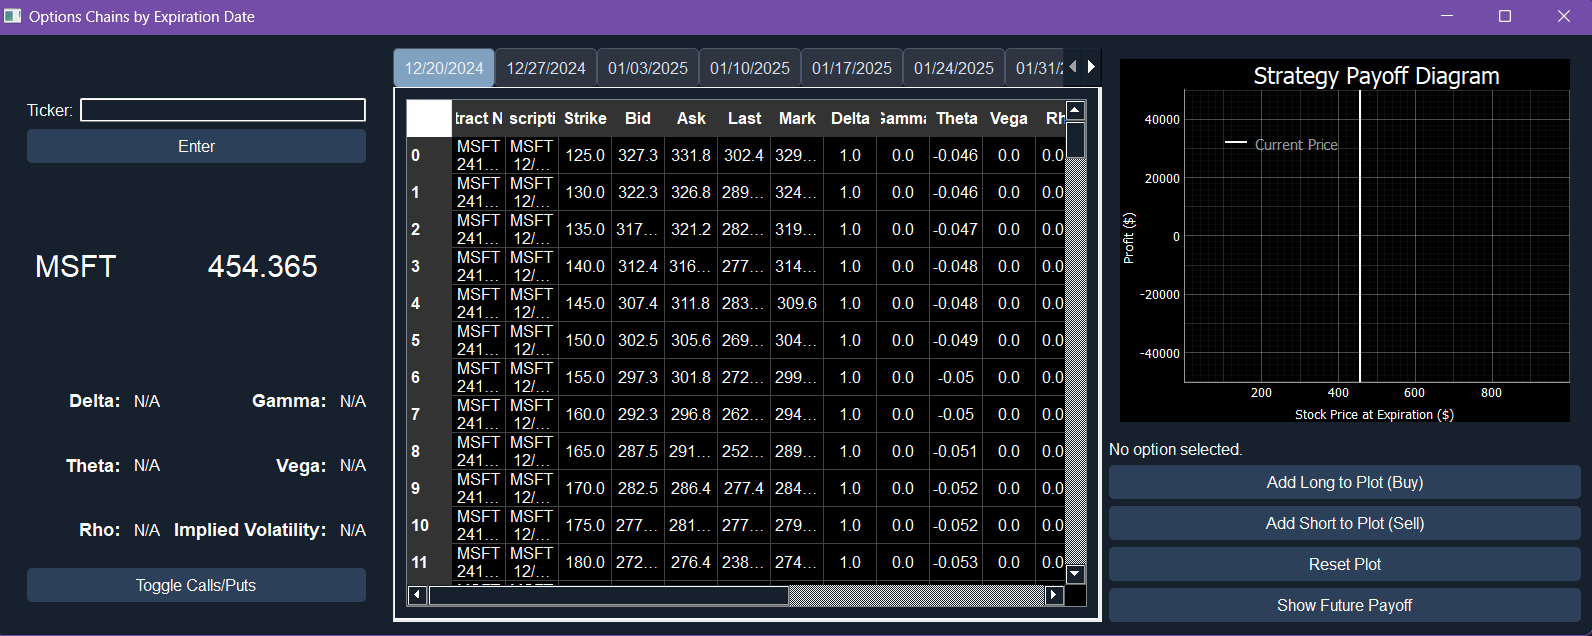
\includegraphics[width=1.4\textwidth]{assets/strategy-builder-stockdata.png}}
    \caption{\label{fig:Figure 8}Initial rendering of the Strategy Builder window with Microsoft data loaded.}
\end{figure}

Note that the middle DataFrame has been populated with the full call options chain for the stock, and different chains for specific days are available for selection on the top. Clicking the \enquote{Toggle Calls/Puts} button will render puts instead. On the left hand side, the current stock price has been loaded, and on the Strategy Payoff Diagram, a vertical line has been drawn to mark the current stock price. 

\indent If we select a long call option expiring on 12/20/2024, at $K=455$ and add it to our plot, our window will populate with options data. This example can be found in Figure \ref{fig:Figure 9}. Unfortunately, pyqtgraph does not have an inherent method of coloring one graph different colors based on a condition. The only way to color the plot green when profit is positive and red when profit is negative is to create two separate lines and attempt to \enquote{merge} them. This unfortunately results in a gap between the two profit lines.   

\begin{figure}[htbp]
    \centering
    \makebox[\textwidth]{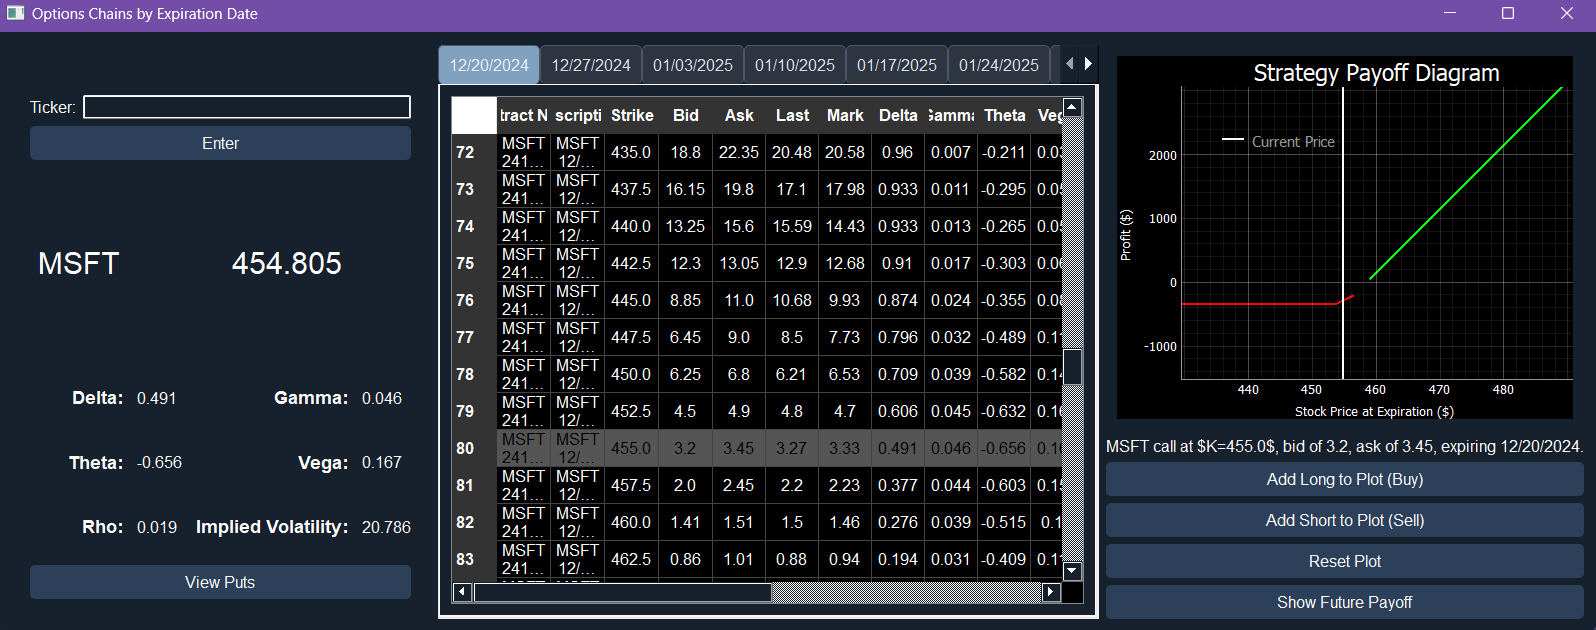
\includegraphics[width=1.4\textwidth]{assets/strategy-builder-optiondata.png}}
    \caption{\label{fig:Figure 9}Strategy Builder window with Microsoft call option, $K=455$, expiring on 12/20/2024.}
\end{figure}

\indent With the long call plotted, the user can next select the \enquote{Show Future Payoff} button to view the calculated payoff of their option strategy in the future. An example is shown in Figure \ref{fig:Figure 10}. The x-axis displays the dates leading up to the expiration of the option strategy, and the y-axis displays the range of prices that have been used to calculate the value. Toggling to profit using the button on the upper-right-hand corner of the window yields the net profit of the position at each datapoint, which is simply the value minus the total cost. The user is also able to adjust the range of prices they would like to see by controlling the Min and Max labels. 

\begin{figure}[htbp]
    \centering
    \makebox[\textwidth]{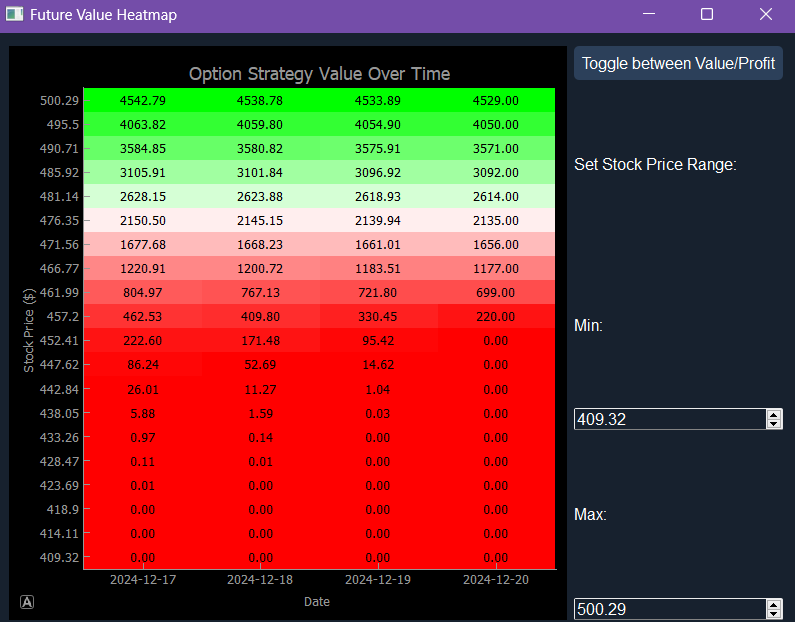
\includegraphics[width=1\textwidth]{assets/heatmap.png}}
    \caption{\label{fig:Figure 10}Future payoff diagram for Microsoft call option, $K=455$, expiring on 12/20/2024.}
\end{figure}

All of the functionality described above can be used with strategies involving multiple options, allowing users to view ranges of maximum profit for advanced strategies. 

\section{Future Work}

\indent Future work for the project will primarily center around cleaning up the interface of the Option Profit Calculator and find ways to improve the design of the UI. This includes finding different ways to plot the options that eliminates the discontinuity in the graph, allowing users to expand or even download the middle DataFrame to better view some of the columns, and using more advanced libraries to organize the button layout and reduce white space. 

\indent Development would also focus on fleshing out the Portfolio Viewer tab. The original vision was to include sections for the user to view statistics around their investments in their trading account, including information about their correlation with the market and risk factors in their portfolio. However, issues and setbacks with rendering graphs in PyQt5 and complications with cleaning up the layout made it infeasible to create the Portfolio Viewer within the timeline of this project.  

\printbibliography

% \begin{thebibliography}{9} % The argument here is the widest label

% \bibitem{lamport1994latex}
%   Leslie Lamport,
%   \textit{LaTeX: A Document Preparation System},
%   Addison-Wesley, 2nd edition, 1994.

% \bibitem{knuth1984texbook}
%   Donald E. Knuth,
%   \textit{The \TeX{}book},
%   Addison-Wesley, 1984.

% \end{thebibliography}



\end{document} 
